\documentclass[10pt,a4paper]{article}
\usepackage[margin=1.65cm,top=1.55cm,bottom=1.55cm,headheight=19pt,headsep=8pt,footskip=22pt]{geometry}
\usepackage[T1]{fontenc}
\usepackage[utf8]{inputenc}
\usepackage{lmodern}
\usepackage{xcolor,graphicx,amsmath,amssymb,array,calc,longtable,booktabs,etoolbox,fancyhdr,hyperref}
\usepackage{microtype}
\usepackage{tikz}
\usetikzlibrary{arrows.meta,calc}
\definecolor{hcmutblue}{HTML}{123A91}
\definecolor{mutedorange}{HTML}{AE6B0C}
\definecolor{answergray}{HTML}{6B6B6B}
\hypersetup{hidelinks,pdfauthor={Teddy Nguyen},pdftitle={Milestone 2 Report: Single-cycle Processor}}
\setlength{\parindent}{0pt}
\setlength{\parskip}{3pt}
\setlength{\emergencystretch}{3em}
\setcounter{secnumdepth}{-1}
\providecommand{\tightlist}{\setlength{\itemsep}{0pt}\setlength{\parskip}{0pt}}
\makeatletter
\patchcmd\longtable{\par}{\if@noskipsec\mbox{}\fi\par}{}{}
\makeatother
\renewcommand{\arraystretch}{1.15}
\setlength{\LTpre}{3pt}
\setlength{\LTpost}{6pt}
\pagestyle{fancy}
\fancyhf{}
\fancyhead[L]{\bfseries Computer Architecture Laboratory - Milestone 2 Report: Single-cycle Processor}
\renewcommand{\headrulewidth}{0.7pt}
\fancyfoot[L]{\nouppercase{\leftmark}}
\fancyfoot[R]{\textcolor{mutedorange}{\thepage}}
\renewcommand{\footrulewidth}{0.7pt}
\renewcommand{\sectionmark}[1]{\markboth{#1}{}}
\renewcommand{\section}[1]{\clearpage\refstepcounter{section}\markboth{#1}{}\vspace*{-0.7em}{\LARGE\bfseries\color{hcmutblue}#1}\par\vspace{0.5em}}
\renewcommand{\subsection}[1]{\markboth{#1}{}\vspace{0.6em}{\Large\bfseries\color{hcmutblue}#1}\par\vspace{0.25em}}
\renewcommand{\subsubsection}[1]{\vspace{0.4em}{\large\bfseries\color{hcmutblue}#1}\par\vspace{0.2em}}
\newcommand{\code}[1]{\texttt{#1}}
\newcommand{\todo}[1]{\textcolor{mutedorange}{\textit{[TODO: #1]}}}
% Include a screenshot if the file exists, otherwise show a TODO box.
\newcommand{\figslot}[2]{%
  \IfFileExists{#1}%
    {\begin{center}\includegraphics[width=\linewidth,height=0.42\textheight,keepaspectratio]{#1}\end{center}}%
    {\begin{center}\fbox{\parbox{0.92\linewidth}{\todo{#2. Save it as \texttt{#1}.}}}\end{center}}}
\newcommand{\logoA}{\IfFileExists{Figures/image1.png}{\includegraphics[width=0.85\linewidth]{Figures/image1.png}}%
  {\IfFileExists{Figures/hcmut.png}{
\includegraphics[width=0.85\linewidth]{Figures/hcmut.png}}{}}}
\newcommand{\logoB}{\IfFileExists{Figures/image2.png}{\includegraphics[width=0.72\linewidth]{Figures/image2.png}}{}}
% Bus-width mark: \bw[label position]{x,y}{width}
\newcommand{\bw}[3][above right]{%
  \draw[thin] ($(#2)+(-0.07,-0.11)$) -- ($(#2)+(0.07,0.11)$);
  \node[font=\tiny,inner sep=1pt,#1] at (#2) {#3};}
% Multiplexer trapezoid: \muxshape{x}{y}{half-height}; select input enters the bottom edge at (x, y-h+0.125)
\newcommand{\muxshape}[3]{%
  \draw[thick, draw=hcmutblue, fill=mutedorange!15] (#1-0.25,#2+#3) -- (#1+0.25,#2+#3-0.25)
    -- (#1+0.25,#2-#3+0.25) -- (#1-0.25,#2-#3) -- cycle;}
% Clock input triangle on the bottom edge of a block: \clkmark{x}{y}
\newcommand{\clkmark}[2]{%
  \draw[thick, draw=hcmutblue] (#1-0.12,#2) -- (#1,#2+0.2) -- (#1+0.12,#2);
  \node[font=\tiny, inner sep=1pt, below] at (#1,#2) {clk};}
% Control signal from the control bar (top edge at y=0) up to a block: \ctlup{x}{y-end}{name}
\newcommand{\ctlup}[3]{%
  \draw[ctl] (#1,0) -- (#1,#2);
  \node[font=\tiny, inner sep=1pt, rotate=90, anchor=south west] at (#1-0.03,0.08) {#3};}
\tikzset{
  blk/.style={draw=hcmutblue, fill=hcmutblue!7, thick, align=center, inner sep=1pt},
  mux/.style={draw=hcmutblue, fill=mutedorange!15, thick, rounded corners=4pt, inner sep=0pt},
  w/.style={-{Latex[length=2mm]}, thick},
  ln/.style={thick},
  ctl/.style={-{Latex[length=2mm]}, densely dashed, thick, mutedorange},
  jn/.style={circle, fill, inner sep=0pt, minimum size=3.2pt},
  lab/.style={font=\tiny, inner sep=1pt}
}
\begin{document}
\begin{titlepage}
\thispagestyle{empty}
\noindent\begin{minipage}[c]{0.13\textwidth}\logoA\end{minipage}%
\begin{minipage}[c]{0.84\textwidth}\bfseries Vietnam National University Ho Chi Minh city\\Ho Chi Minh city University of Technology\end{minipage}
\vspace{1mm}\hrule height 0.7pt
\vfill
\begin{center}
{\LARGE\bfseries Computer Architecture Laboratory\par}\vspace{3mm}
{\large Milestone 2 Report: Single-cycle Processor\par}
\end{center}
\vspace{1.2cm}
\begin{center}\begin{tabular}{@{}>{\bfseries}p{0.22\textwidth}p{0.52\textwidth}@{}}
Status: & Report, Version 1.0\\
Group: & 09\\
Members: & Ho Ngoc Cuong - 2570082\\
& Nguyen Xuan Nam - 2570462\\
Instructors: & Khai Pham, Vy Luong\\
Date: & 2026-Nov-07\\
\end{tabular}\end{center}
\vfill
\hrule height 0.7pt\vspace{2mm}
\noindent\begin{minipage}[c]{0.10\textwidth}\logoB\end{minipage}%
\begin{minipage}[c]{0.86\textwidth}\bfseries D.O.E Lab\\Department of Electronics\end{minipage}
\end{titlepage}

\section{1. Work Distribution}

\textbf{Table 1:} Contribution of each member (total 100\%).

\begin{tabular}{@{}p{0.24\linewidth}p{0.16\linewidth}p{0.37\linewidth}p{0.14\linewidth}@{}}
\toprule
\textbf{Member} & \textbf{Student ID} & \textbf{Tasks} & \textbf{Contribution (\%)} \\
\midrule
Ho Ngoc Cuong & 2570082 & Investigation, RTL development, simulation and testing & 50\% \\
Nguyen Xuan Nam & 2570462 & Investigation, RTL development, report & 50\% \\
\bottomrule
\end{tabular}

\section{2. Result Summary}

Fill in the numbers from the SIMULATION SUMMARY printed at the end of
each run.

\textbf{Table 2:} ISA\_TEST results.

\begin{tabular}{@{}p{0.35\linewidth}p{0.6\linewidth}@{}}
\toprule
\textbf{Metric} & \textbf{Your result} \\
\midrule
Total tests passed & 37 / 37 \\
Check groups passed & 86 / 86 \\
Total cases passed & 404988 / 404988 \\
Total cycles & 5497867 \\
Total instructions & 5497867 \\
IPC & 1.0000 \\
ISA score & 6.00 / 6.00 \\
\bottomrule
\end{tabular}

\textbf{Figure 1:} ISA\_TEST simulation summary.

\figslot{Figures/isa-summary.png}{paste a screenshot of the ISA\_TEST SIMULATION SUMMARY (values in Table 2)}

\textbf{Table 3:} C program results (at least three must pass).

\begin{tabular}{@{}p{0.22\linewidth}p{0.27\linewidth}p{0.14\linewidth}p{0.14\linewidth}p{0.09\linewidth}@{}}
\toprule
\textbf{Program} & \textbf{Result (PASS / FAIL / not run)} & \textbf{Cycles} & \textbf{Instructions} & \textbf{IPC} \\
\midrule
PROG\_HANOI & PASS (4095/4095 moves) & 339657 & 339657 & 1.0000 \\
PROG\_SORT & PASS (6/6 algorithms) & 486758 & 486758 & 1.0000 \\
PROG\_MATRIX & PASS (0 cross-check errors) & 171393 & 171393 & 1.0000 \\
PROG\_SOFTFLOAT & PASS (56/56) & 2857414 & 2857414 & 1.0000 \\
PROG\_SIGMOID & PASS (62/62) & 3822619 & 3822619 & 1.0000 \\
PROG\_CONVOLUTION & PASS (125/125) & 1811378 & 1811378 & 1.0000 \\
\bottomrule
\end{tabular}

\textbf{Figure 2:} Console output of a C program.

\figslot{Figures/c-console.png}{paste a screenshot of the console output of one C program, e.g. PROG\_HANOI}

\textbf{Q2.1 Which test groups or programs fail, and what is the cause
you found or suspect? Write "None" if all pass.}

None. All 37 ISA instruction tests (86 check groups, 404988 cases) and all six
C programs pass. Every test was run with both \code{IMEM\_FORMAT=1B} and
\code{IMEM\_FORMAT=4B}; both formats give the same results and the same cycle
counts. In every run the testbench ends with \code{\$finish}, with no timeout.

\section{3. Design}

\subsection{3.1. Datapath}

\textbf{Figure 3:} Implemented single-cycle datapath.

\begin{center}
\resizebox{\linewidth}{!}{%
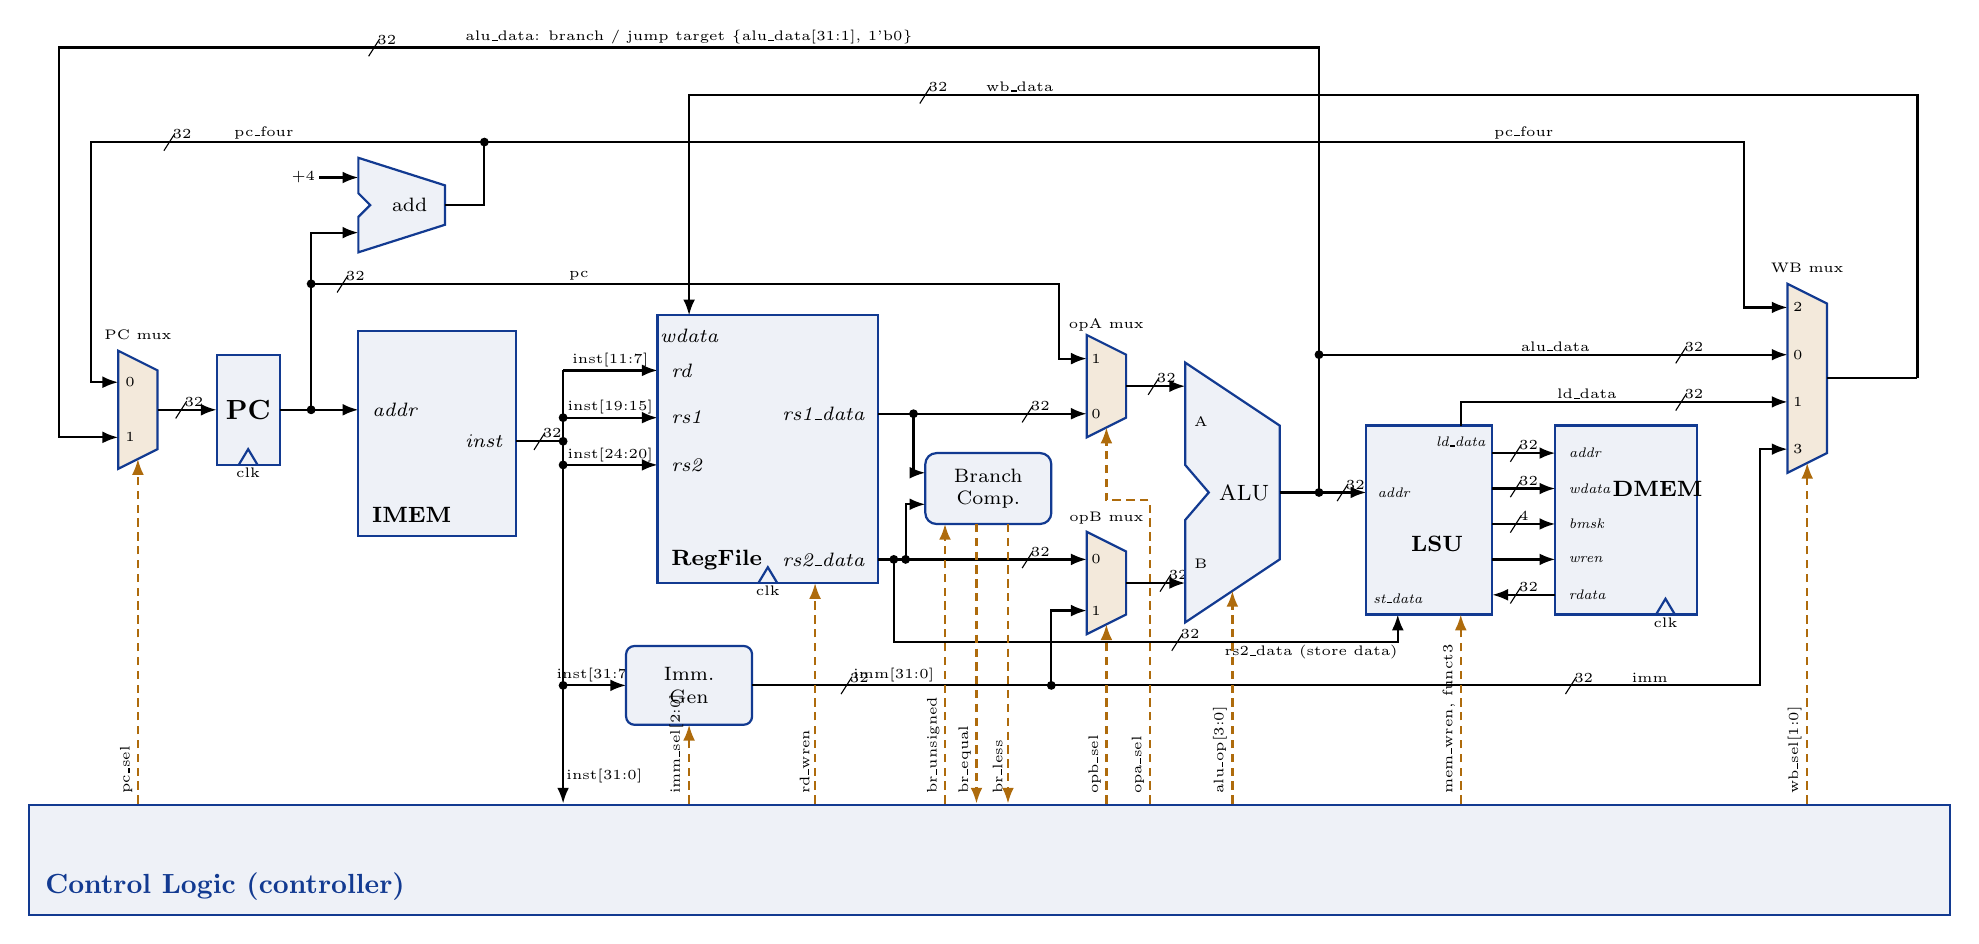
\begin{tikzpicture}[font=\scriptsize]
  % ================= Control logic bar (top edge at y = 0) =================
  \node[draw=hcmutblue, fill=hcmutblue!7, thick, minimum width=24.4cm, minimum height=1.4cm,
        anchor=north west, inner sep=0pt] (ctrl) at (-1.4,0) {};
  \node[anchor=south west, font=\normalsize\bfseries, text=hcmutblue] at (-1.3,-1.35) {Control Logic (controller)};

  % ================= PC mux, PC register, PC+4 adder =================
  \muxshape{0}{5.0}{0.75}
  \node[lab] at (-0.1,5.35) {0}; \node[lab] at (-0.1,4.65) {1};
  \node[lab, above] at (0,5.85) {PC mux};
  \node[blk, minimum width=8mm, minimum height=14mm, font=\bfseries] (pc) at (1.4,5.0) {PC};
  \clkmark{1.4}{4.3}
  \draw[w] (0.25,5.0) -- (1.0,5.0); \bw{0.55,5.0}{32}
  \draw[ln] (1.8,5.0) -- (2.2,5.0); \node[jn] at (2.2,5.0) {};
  \draw[w] (2.2,5.0) -- (2.8,5.0);
  \draw[w] (2.2,5.0) -- (2.2,7.25) -- (2.8,7.25);
  \draw[w] (2.3,7.95) node[lab, left] {+4} -- (2.8,7.95);
  \draw[thick, draw=hcmutblue, fill=hcmutblue!7] (2.8,8.2) -- (3.9,7.85) -- (3.9,7.35) -- (2.8,7.0)
    -- (2.8,7.45) -- (2.95,7.6) -- (2.8,7.75) -- cycle;
  \node at (3.45,7.6) {add};
  % pc_four: back to PC mux (0) and to write-back mux (2)
  \draw[ln] (3.9,7.6) -- (4.4,7.6) -- (4.4,8.4); \node[jn] at (4.4,8.4) {};
  \draw[w] (4.4,8.4) -- (-0.6,8.4) -- (-0.6,5.35) -- (-0.25,5.35);
  \draw[w] (4.4,8.4) -- (20.4,8.4) -- (20.4,6.3) -- (20.95,6.3);
  \bw{0.4,8.4}{32} \node[lab, above] at (1.6,8.4) {pc\_four};
  \node[lab, above] at (17.6,8.4) {pc\_four};

  % ================= IMEM =================
  \node[blk, minimum width=20mm, minimum height=26mm] (imem) at (3.8,4.7) {};
  \node[anchor=west, font=\scriptsize\itshape] at (2.85,5.0) {addr};
  \node[anchor=east, font=\scriptsize\itshape] at (4.75,4.6) {inst};
  \node[anchor=south west, font=\footnotesize\bfseries] at (2.85,3.45) {IMEM};

  % pc to operand-A mux (input 1)
  \node[jn] at (2.2,6.6) {};
  \draw[w] (2.2,6.6) -- (11.7,6.6) -- (11.7,5.65) -- (12.05,5.65);
  \bw{2.6,6.6}{32} \node[lab, above] at (5.6,6.6) {pc};

  % ================= Instruction bus =================
  \draw[ln] (4.8,4.6) -- (5.4,4.6); \node[jn] at (5.4,4.6) {};
  \bw{5.1,4.6}{32}
  \draw[w] (5.4,5.5) -- (5.4,0);
  \node[lab, right] at (5.4,0.35) {inst[31:0]};
  \draw[w] (5.4,5.5) -- (6.6,5.5);                       \node[lab, above] at (6.0,5.5) {inst[11:7]};
  \node[jn] at (5.4,4.9) {}; \draw[w] (5.4,4.9) -- (6.6,4.9); \node[lab, above] at (6.0,4.9) {inst[19:15]};
  \node[jn] at (5.4,4.3) {}; \draw[w] (5.4,4.3) -- (6.6,4.3); \node[lab, above] at (6.0,4.3) {inst[24:20]};
  \node[jn] at (5.4,1.5) {}; \draw[w] (5.4,1.5) -- (6.2,1.5); \node[lab, above] at (5.8,1.5) {inst[31:7]};

  % ================= Register file =================
  \node[blk, minimum width=28mm, minimum height=34mm] (rf) at (8.0,4.5) {};
  \node[anchor=north, font=\scriptsize\itshape] at (7.0,6.15) {wdata};
  \node[anchor=west, font=\scriptsize\itshape] at (6.65,5.5) {rd};
  \node[anchor=west, font=\scriptsize\itshape] at (6.65,4.9) {rs1};
  \node[anchor=west, font=\scriptsize\itshape] at (6.65,4.3) {rs2};
  \node[anchor=east, font=\scriptsize\itshape] at (9.35,4.95) {rs1\_data};
  \node[anchor=east, font=\scriptsize\itshape] at (9.35,3.1) {rs2\_data};
  \node[anchor=south west, font=\footnotesize\bfseries] at (6.65,2.85) {RegFile};
  \clkmark{8.0}{2.8}

  % ================= Immediate generator =================
  \node[blk, rounded corners=3pt, minimum width=16mm, minimum height=10mm] (immg) at (7.0,1.5) {Imm.\\Gen};
  \draw[ln] (7.8,1.5) -- (11.6,1.5); \node[jn] at (11.6,1.5) {};
  \bw{9.0,1.5}{32} \node[lab, above] at (9.6,1.5) {imm[31:0]};
  \draw[w] (11.6,1.5) -- (11.6,2.45) -- (12.05,2.45);
  \draw[w] (11.6,1.5) -- (20.6,1.5) -- (20.6,4.5) -- (20.95,4.5);
  \bw{18.2,1.5}{32} \node[lab, above] at (19.2,1.5) {imm};

  % ================= Register outputs and branch comparator =================
  \node[blk, rounded corners=4pt, minimum width=16mm, minimum height=9mm] (bc) at (10.8,4.0) {Branch\\Comp.};
  \draw[w] (9.4,4.95) -- (12.05,4.95); \bw{11.3,4.95}{32}
  \node[jn] at (9.85,4.95) {}; \draw[w] (9.85,4.95) -- (9.85,4.2) -- (10.0,4.2);
  \draw[w] (9.4,3.1) -- (12.05,3.1);   \bw{11.3,3.1}{32}
  \node[jn] at (9.75,3.1) {}; \draw[w] (9.75,3.1) -- (9.75,3.8) -- (10.0,3.8);
  % rs2_data to the LSU as store data
  \node[jn] at (9.6,3.1) {}; \draw[w] (9.6,3.1) -- (9.6,2.05) -- (16.0,2.05) -- (16.0,2.4);
  \bw{13.2,2.05}{32} \node[lab, below] at (14.9,2.05) {rs2\_data (store data)};

  % ================= Operand muxes =================
  \muxshape{12.3}{5.3}{0.65}
  \node[lab] at (12.17,5.65) {1}; \node[lab] at (12.17,4.95) {0};
  \node[lab, above] at (12.3,5.95) {opA mux};
  \muxshape{12.3}{2.8}{0.65}
  \node[lab] at (12.17,3.1) {0}; \node[lab] at (12.17,2.45) {1};
  \node[lab] at (12.3,3.63) {opB mux};
  \draw[w] (12.55,5.3) -- (13.3,5.3); \bw{12.9,5.3}{32}
  \draw[w] (12.55,2.8) -- (13.3,2.8); \bw{13.05,2.8}{32}

  % ================= ALU =================
  \draw[thick, draw=hcmutblue, fill=hcmutblue!7] (13.3,5.6) -- (14.5,4.8) -- (14.5,3.1) -- (13.3,2.3)
    -- (13.3,3.6) -- (13.6,3.95) -- (13.3,4.3) -- cycle;
  \node[font=\footnotesize] at (14.05,3.95) {ALU};
  \node[lab] at (13.5,4.85) {A}; \node[lab] at (13.5,3.05) {B};
  \draw[ln] (14.5,3.95) -- (15.0,3.95); \node[jn] at (15.0,3.95) {};
  \draw[w] (15.0,3.95) -- (15.6,3.95); \bw{15.3,3.95}{32}
  % alu_data: branch/jump target back to the PC mux (1)
  \draw[w] (15.0,3.95) -- (15.0,9.6) -- (-1.0,9.6) -- (-1.0,4.65) -- (-0.25,4.65);
  \bw{3.0,9.6}{32} \node[lab, above] at (7.0,9.6) {alu\_data: branch / jump target \{alu\_data[31:1], 1'b0\}};
  % alu_data to the write-back mux (0)
  \node[jn] at (15.0,5.7) {}; \draw[w] (15.0,5.7) -- (20.95,5.7);
  \bw{19.6,5.7}{32} \node[lab, above] at (18.0,5.7) {alu\_data};

  % ================= LSU and DMEM =================
  \node[blk, minimum width=16mm, minimum height=24mm] (lsu) at (16.4,3.6) {};
  \node[font=\footnotesize\bfseries] at (16.5,3.3) {LSU};
  \node[anchor=west, font=\tiny\itshape] at (15.62,3.95) {addr};
  \node[anchor=south, font=\tiny\itshape] at (16.0,2.42) {st\_data};
  \node[anchor=north, font=\tiny\itshape] at (16.8,4.78) {ld\_data};
  \node[blk, minimum width=18mm, minimum height=24mm] (dmem) at (18.9,3.6) {};
  \node[font=\footnotesize\bfseries] at (19.3,4.0) {DMEM};
  \foreach \y/\n in {4.45/addr, 4.0/wdata, 3.55/bmsk, 3.1/wren, 2.65/rdata}
    {\node[anchor=west, font=\tiny\itshape] at (18.05,\y) {\n};}
  \foreach \y in {4.45, 4.0, 3.55, 3.1} {\draw[w] (17.2,\y) -- (18.0,\y);}
  \draw[w] (18.0,2.65) -- (17.2,2.65);
  \bw{17.5,4.45}{32} \bw{17.5,4.0}{32} \bw{17.5,3.55}{4} \bw{17.5,2.65}{32}
  \clkmark{19.4}{2.4}
  % ld_data to the write-back mux (1)
  \draw[w] (16.8,4.8) -- (16.8,5.1) -- (20.95,5.1);
  \bw{19.6,5.1}{32} \node[lab, above] at (18.4,5.1) {ld\_data};

  % ================= Write-back mux =================
  \muxshape{21.2}{5.4}{1.2}
  \node[lab] at (21.08,6.3) {2}; \node[lab] at (21.08,5.7) {0};
  \node[lab] at (21.08,5.1) {1}; \node[lab] at (21.08,4.5) {3};
  \node[lab, above] at (21.2,6.7) {WB mux};
  \draw[ln] (21.45,5.4) -- (22.6,5.4);
  \draw[w] (22.6,5.4) -- (22.6,9.0) -- (7.0,9.0) -- (7.0,6.2);
  \bw{10.0,9.0}{32} \node[lab, above] at (11.2,9.0) {wb\_data};

  % ================= Control signals =================
  \ctlup{0}{4.375}{pc\_sel}
  \ctlup{7.0}{1.0}{imm\_sel[2:0]}
  \ctlup{8.6}{2.8}{rd\_wren}
  \ctlup{10.25}{3.55}{br\_unsigned}
  \draw[ctl] (10.65,3.55) -- (10.65,0);
  \node[lab, rotate=90, anchor=south west] at (10.62,0.08) {br\_equal};
  \draw[ctl] (11.05,3.55) -- (11.05,0);
  \node[lab, rotate=90, anchor=south west] at (11.02,0.08) {br\_less};
  \ctlup{12.3}{2.275}{opb\_sel}
  \draw[ctl] (12.85,0) -- (12.85,3.85) -- (12.3,3.85) -- (12.3,4.775);
  \node[lab, rotate=90, anchor=south west] at (12.82,0.08) {opa\_sel};
  \ctlup{13.9}{2.7}{alu\_op[3:0]}
  \ctlup{16.8}{2.4}{mem\_wren, funct3}
  \ctlup{21.2}{4.325}{wb\_sel[1:0]}
\end{tikzpicture}}
\end{center}

{\small Solid lines are data. Dashed lines are control signals between the
control logic (bottom) and the datapath; \code{br\_equal} and \code{br\_less}
go from the branch comparator to the control logic, all others go from the
control logic to the datapath. A slash with a number gives the bus width; unmarked lines are
1 bit. Numbers inside a multiplexer are its select values. The register
fields are rs1 = \code{instr[19:15]}, rs2 = \code{instr[24:20]},
rd = \code{instr[11:7]} and funct3 = \code{instr[14:12]}. The PC, the register
file and DMEM are written on the rising clock edge; all other paths are
combinational.\par}

\textbf{Q3.1 List the modules of your processor and the role of each,
and explain how they connect to form the datapath in Figure 3.}

\begin{tabular}{@{}p{0.2\linewidth}p{0.46\linewidth}p{0.28\linewidth}@{}}
\toprule
\textbf{Module} & \textbf{Role} & \textbf{Connects to} \\
\midrule
\code{milestone2} (TA wrapper) & Instantiates core, IMEM and DMEM; decodes MMIO stores (print, ISA, halt). & Core, IMEM, DMEM, testbench \\
\code{singlecycle} & Top core: PC register, PC+4 adder, next-PC mux, opA/opB muxes, write-back mux. Instantiates all submodules. & All submodules, IMEM address, DMEM bus \\
\code{controller} & Decodes \code{instr}, checks encoding validity, drives all control signals. & \code{instr} from IMEM; BRC outputs in; control to every block \\
\code{immgen} & Builds the I, S, B, U and J immediates. & \code{instr}; output to opB mux \\
\code{regfile} & 32 x 32-bit registers, two asynchronous reads (rs1, rs2), one synchronous write (rd). & \code{instr} fields; rs1/rs2 to BRC, ALU and LSU; write-back data in \\
\code{brc} (uses \code{comparator}) & Computes \code{equal} and \code{less} of rs1 and rs2 for branches. & Register file in; controller out \\
\code{alu} (\code{adder}, \code{comparator}, \code{shifter}) & Ten integer operations; also computes memory addresses and branch/jump targets. & opA/opB muxes in; LSU address, next-PC mux, write-back mux out \\
\code{lsu} & Store alignment and byte mask; load byte/half selection and extension. & ALU result (address), rs2 (store data), DMEM, write-back mux \\
\code{imem} & Instruction memory, asynchronous read. & PC in; \code{instr} out \\
\code{dmem} & Data memory, asynchronous read, synchronous byte-masked write. & LSU in/out \\
\bottomrule
\end{tabular}

The PC drives IMEM. The controller and immgen decode the instruction in the
same cycle, and the register file reads rs1 and rs2. The opA mux selects rs1
or PC, and the opB mux selects rs2 or the immediate. The ALU then produces an
arithmetic/logic result, a memory address, or a branch/jump target. The LSU
forwards the address to DMEM and aligns load data. The write-back mux selects
ALU, load, PC+4 or immediate data for the register file. The next-PC mux
selects PC+4 or the ALU target when \code{pc\_sel} is set.

\subsection{3.2. Implementation}

\textbf{Q3.2 Arithmetic, logic and shift operations.}

\begin{center}
\resizebox{0.9\linewidth}{!}{%
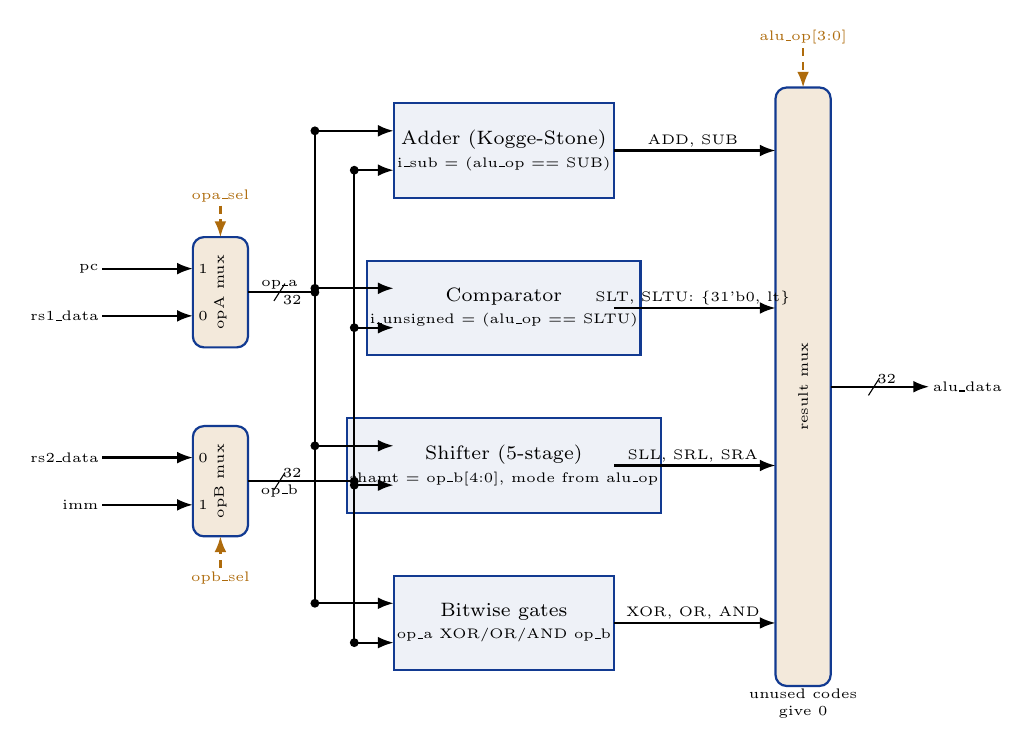
\begin{tikzpicture}[font=\scriptsize]
  \node[mux, minimum width=7mm, minimum height=14mm] (am) at (0,1.2) {\rotatebox{90}{\tiny opA mux}};
  \node[lab] at (-0.22,1.5) {1}; \node[lab] at (-0.22,0.9) {0};
  \node[mux, minimum width=7mm, minimum height=14mm] (bm) at (0,-1.2) {\rotatebox{90}{\tiny opB mux}};
  \node[lab] at (-0.22,-0.9) {0}; \node[lab] at (-0.22,-1.5) {1};
  \draw[w] (-1.5,1.5) node[lab, left] {pc} -- (-0.35,1.5);
  \draw[w] (-1.5,0.9) node[lab, left] {rs1\_data} -- (-0.35,0.9);
  \draw[w] (-1.5,-0.9) node[lab, left] {rs2\_data} -- (-0.35,-0.9);
  \draw[w] (-1.5,-1.5) node[lab, left] {imm} -- (-0.35,-1.5);
  \draw[ctl] (0,2.3) node[lab, above] {opa\_sel} -- (0,1.9);
  \draw[ctl] (0,-2.3) node[lab, below] {opb\_sel} -- (0,-1.9);

  \node[blk, minimum width=28mm, minimum height=12mm] (add) at (3.6,3.0)
    {Adder (Kogge-Stone)\\\tiny i\_sub = (alu\_op == SUB)};
  \node[blk, minimum width=28mm, minimum height=12mm] (cmp) at (3.6,1.0)
    {Comparator\\\tiny i\_unsigned = (alu\_op == SLTU)};
  \node[blk, minimum width=28mm, minimum height=12mm] (sh) at (3.6,-1.0)
    {Shifter (5-stage)\\\tiny shamt = op\_b[4:0], mode from alu\_op};
  \node[blk, minimum width=28mm, minimum height=12mm] (lg) at (3.6,-3.0)
    {Bitwise gates\\\tiny op\_a XOR/OR/AND op\_b};

  % op_a and op_b buses
  \draw[ln] (0.35,1.2) -- (1.2,1.2); \node[jn] at (1.2,1.2) {};
  \draw[ln] (1.2,3.25) -- (1.2,-2.75);
  \draw[ln] (0.35,-1.2) -- (1.7,-1.2); \node[jn] at (1.7,-1.2) {};
  \draw[ln] (1.7,2.75) -- (1.7,-3.25);
  \foreach \y in {3.0,1.0,-1.0,-3.0} {
    \node[jn] at (1.2,\y+0.25) {}; \draw[w] (1.2,\y+0.25) -- (2.2,\y+0.25);
    \node[jn] at (1.7,\y-0.25) {}; \draw[w] (1.7,\y-0.25) -- (2.2,\y-0.25);
  }
  \node[lab, above] at (0.75,1.2) {op\_a}; \bw[below right]{0.75,1.2}{32}
  \node[lab, below] at (0.75,-1.2) {op\_b}; \bw{0.75,-1.2}{32}

  \node[mux, minimum width=7mm, minimum height=76mm] (rm) at (7.4,0) {\rotatebox{90}{\tiny result mux}};
  \draw[w] (5.0,3.0) -- (7.05,3.0);   \node[lab, above] at (6.0,3.0) {ADD, SUB};
  \draw[w] (5.0,1.0) -- (7.05,1.0);   \node[lab, above] at (6.0,1.0) {SLT, SLTU: \{31'b0, lt\}};
  \draw[w] (5.0,-1.0) -- (7.05,-1.0); \node[lab, above] at (6.0,-1.0) {SLL, SRL, SRA};
  \draw[w] (5.0,-3.0) -- (7.05,-3.0); \node[lab, above] at (6.0,-3.0) {XOR, OR, AND};
  \draw[ctl] (7.4,4.3) node[lab, above] {alu\_op[3:0]} -- (7.4,3.8);
  \node[lab, below, align=center] at (7.4,-3.8) {unused codes\\give 0};
  \draw[w] (7.75,0) -- (9.0,0) node[lab, right] {alu\_data}; \bw{8.3,0}{32}
\end{tikzpicture}}
\end{center}

The ALU in \code{alu.sv} uses one adder, one comparator and one shifter, and
selects the result with a 4-bit \code{alu\_op}. \code{adder.sv} is a 32-bit
Kogge-Stone prefix adder. Subtraction inverts \code{b} and injects a carry-in
of 1. It computes ADD and SUB, and also the AUIPC result and the addresses for
load/store, branches, JAL and JALR. The PC+4 value uses a separate adder in \code{singlecycle.sv}.
\code{comparator.sv} is a leading-difference magnitude comparator, with an
unsigned mode for SLTU. It drives the SLT and SLTU results, and the BRC reuses
it. \code{shifter.sv} is a 5-stage logarithmic barrel shifter. Left shifts are
done by bit-reversing the input and output around one right-shifter. The
arithmetic right shift fills with the sign bit. The shift amount is
\code{op\_b[4:0]}. XOR, OR and AND are direct bitwise gates. The operand muxes
select rs1 or PC for opA, and rs2 or the immediate for opB.

\textbf{Q3.3 Branch comparison and selection of the next PC.}

\begin{center}
\resizebox{\linewidth}{!}{%
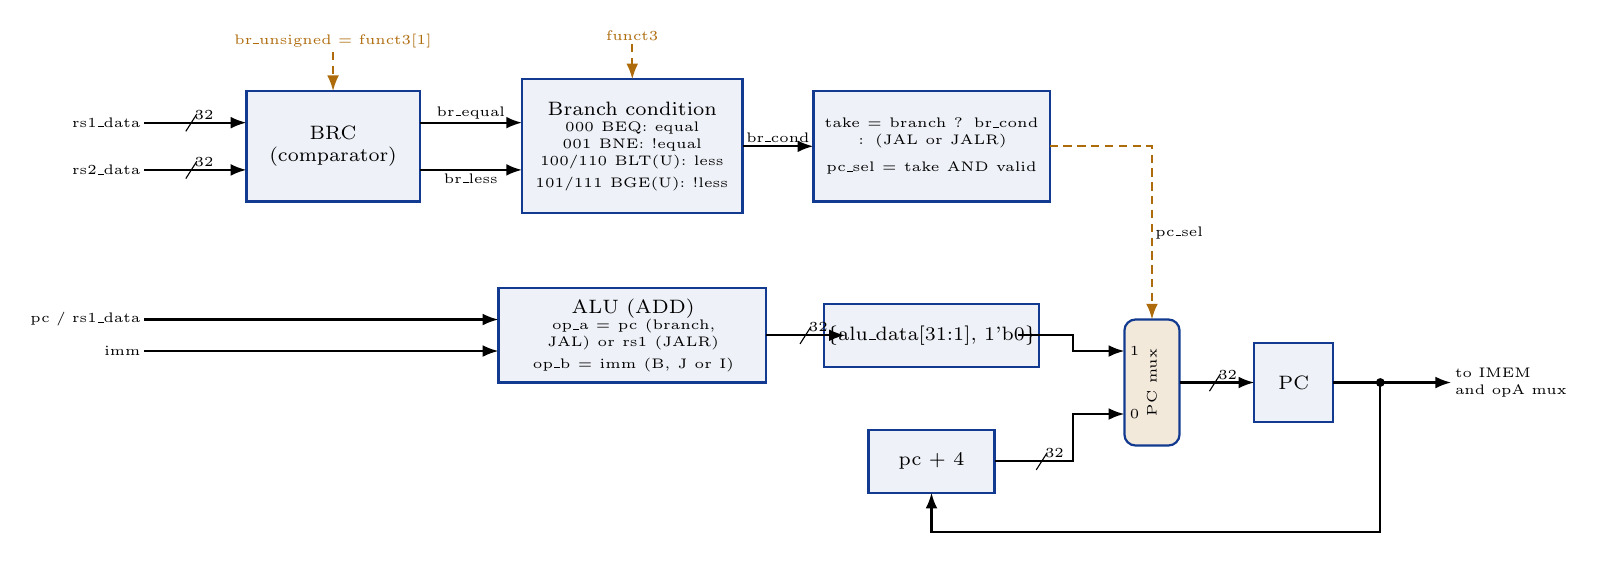
\begin{tikzpicture}[font=\scriptsize]
  % Branch decision
  \node[blk, minimum width=22mm, minimum height=14mm] (brc) at (0,0) {BRC\\(comparator)};
  \draw[w] (-2.4,0.3) node[lab, left] {rs1\_data} -- (-1.1,0.3); \bw{-1.8,0.3}{32}
  \draw[w] (-2.4,-0.3) node[lab, left] {rs2\_data} -- (-1.1,-0.3); \bw{-1.8,-0.3}{32}
  \draw[ctl] (0,1.2) node[lab, above] {br\_unsigned = funct3[1]} -- (0,0.7);
  \node[blk, minimum width=28mm, minimum height=17mm, text width=27mm] (cond) at (3.8,0)
    {Branch condition\\\tiny
     000 BEQ: equal\\001 BNE: !equal\\100/110 BLT(U): less\\101/111 BGE(U): !less};
  \draw[w] (1.1,0.3) -- (2.4,0.3) node[lab, pos=0.5, above] {br\_equal};
  \draw[w] (1.1,-0.3) -- (2.4,-0.3) node[lab, pos=0.5, below] {br\_less};
  \draw[ctl] (3.8,1.3) node[lab, above] {funct3} -- (3.8,0.85);
  \node[blk, minimum width=30mm, minimum height=14mm, text width=29mm] (take) at (7.6,0)
    {\tiny take = branch ? br\_cond : (JAL or JALR)\\[2pt]
     pc\_sel = take AND valid};
  \draw[w] (5.2,0) -- (6.1,0) node[lab, pos=0.5, above] {br\_cond};

  % Target and PC+4
  \node[blk, minimum width=34mm, minimum height=12mm, text width=33mm] (alu) at (3.8,-2.4)
    {ALU (ADD)\\\tiny op\_a = pc (branch, JAL) or rs1 (JALR)\\op\_b = imm (B, J or I)};
  \draw[w] (-2.4,-2.2) node[lab, left] {pc / rs1\_data} -- (2.1,-2.2);
  \draw[w] (-2.4,-2.6) node[lab, left] {imm} -- (2.1,-2.6);
  \node[blk, minimum width=22mm, minimum height=8mm] (clr) at (7.6,-2.4) {\{alu\_data[31:1], 1'b0\}};
  \draw[w] (5.5,-2.4) -- (6.5,-2.4); \bw{6.0,-2.4}{32}
  \node[blk, minimum width=16mm, minimum height=8mm] (add4) at (7.6,-4.0) {pc + 4};

  % Next-PC mux and PC register
  \node[mux, minimum width=7mm, minimum height=16mm] (pcmux) at (10.4,-3.0) {\rotatebox{90}{\tiny PC mux}};
  \node[lab] at (10.18,-2.6) {1}; \node[lab] at (10.18,-3.4) {0};
  \draw[w] (8.7,-2.4) -- (9.4,-2.4) -- (9.4,-2.6) -- (10.05,-2.6);
  \draw[w] (8.4,-4.0) -- (9.4,-4.0) -- (9.4,-3.4) -- (10.05,-3.4); \bw{9.0,-4.0}{32}
  \draw[ctl] (9.1,0) -- (10.4,0) -- (10.4,-2.2);
  \node[lab, right] at (10.4,-1.1) {pc\_sel};
  \node[blk, minimum width=10mm, minimum height=10mm] (pc) at (12.2,-3.0) {PC};
  \draw[w] (10.75,-3.0) -- (11.7,-3.0); \bw{11.2,-3.0}{32}
  \draw[ln] (12.7,-3.0) -- (13.3,-3.0); \node[jn] at (13.3,-3.0) {};
  \draw[w] (13.3,-3.0) -- (14.2,-3.0) node[lab, right, align=left] {to IMEM\\and opA mux};
  \draw[w] (13.3,-3.0) -- (13.3,-4.9) -- (7.6,-4.9) -- (7.6,-4.4);
\end{tikzpicture}}
\end{center}

\code{brc.sv} reuses the \code{comparator} on rs1 and rs2 and outputs
\code{o\_br\_equal} and \code{o\_br\_less}. The controller sets
\code{o\_br\_unsigned = funct3[1]}, which selects signed or unsigned compare.
The controller then selects the condition with \code{funct3}: BEQ uses equal,
BNE uses not-equal, BLT and BLTU use less, and BGE and BGEU use not-less.
The branch is taken only when this condition holds and the instruction is
valid. In the same cycle, the ALU computes the target as PC + immediate, with
opA = PC and opB = immediate. The next-PC mux selects
\code{\{alu\_data[31:1], 1'b0\}} when \code{pc\_sel} is 1, and PC+4 otherwise.
Clearing bit 0 is required for JALR. For branches and JAL it has no effect,
because their targets are always even.

\textbf{Q3.4 Immediate generation for every instruction format.}

\begin{tabular}{@{}p{0.08\linewidth}p{0.30\linewidth}p{0.36\linewidth}p{0.17\linewidth}@{}}
\toprule
\textbf{Format} & \textbf{Instructions} & \textbf{Immediate bits} & \textbf{Extension} \\
\midrule
I & JALR, loads, OP-IMM (ADDI, SLTI[U], XORI, ORI, ANDI, SLLI, SRLI, SRAI) & \code{inst[31:20]} & Sign-extended \\
S & SB, SH, SW & \code{inst[31:25], inst[11:7]} & Sign-extended \\
B & BEQ, BNE, BLT, BGE, BLTU, BGEU & \code{inst[31], inst[7], inst[30:25], inst[11:8], 0} & Sign-extended \\
U & LUI, AUIPC & \code{inst[31:12], 12'b0} & Upper 20 bits \\
J & JAL & \code{inst[31], inst[19:12], inst[20], inst[30:21], 0} & Sign-extended \\
\bottomrule
\end{tabular}

\code{immgen.sv} is a 3-bit \code{imm\_sel} multiplexer over five fixed wire
permutations, with sign extension from \code{inst[31]}. Bit 0 of the B and J
immediates is wired to 0. The shift amount for SLLI, SRLI and SRAI comes from
the I-format immediate, and only \code{imm[4:0]} reaches the shifter.

\textbf{Q3.5 Store data and byte mask for byte, halfword and word
stores; load data for byte, halfword and word loads.}

\begin{tabular}{@{}p{0.10\linewidth}p{0.20\linewidth}p{0.24\linewidth}p{0.38\linewidth}@{}}
\toprule
\textbf{Access} & \textbf{Address bits} & \textbf{Byte mask (\code{bmsk})} & \textbf{Store data / load result} \\
\midrule
SB & \code{addr[1:0]} = 00, 01, 10, 11 & 0001, 0010, 0100, 1000 & \code{rs2[7:0]} replicated to 4 lanes. LB: sign-extended byte. LBU: zero-extended byte. \\
SH & \code{addr[1]} = 0 or 1 & 0011 (\code{addr[1]}=0), 1100 (\code{addr[1]}=1) & \code{rs2[15:0]} replicated to 2 lanes. LH: sign-extended half. LHU: zero-extended half. \\
SW & \code{addr[1:0]} = 00 & 1111 & \code{rs2[31:0]}. LW: full word. \\
Non-store & -- & 0000 & -- \\
\bottomrule
\end{tabular}

DMEM always returns the aligned 32-bit word that contains the address. For
loads, the LSU uses \code{addr[1:0]} to select the byte, and \code{addr[1]} to
select the halfword. A \code{funct3} mux then applies sign or zero extension.
For stores, the LSU replicates the data into every byte lane, and the byte
mask decides which lanes DMEM actually writes. Misaligned halfword and word
accesses are not detected (see Q5.1).

\textbf{Q3.6 Generation of the control signals from the instruction
fields.}

\begin{center}
\resizebox{\linewidth}{!}{%
\begin{tabular}{@{}lccccccccc@{}}
\toprule
\textbf{Type (opcode)} & \textbf{imm\_sel} & \textbf{opa\_sel} & \textbf{opb\_sel} & \textbf{alu\_op} & \textbf{wb\_sel} & \textbf{rd\_wren} & \textbf{mem\_wren} & \textbf{pc\_sel} & \textbf{valid} \\
\midrule
R-type (0110011) & -- & rs1 (0) & rs2 (0) & alu\_f3 & ALU (0) & 1 & 0 & 0 & 1 \\
OP-IMM (0010011) & I (0) & rs1 (0) & imm (1) & alu\_f3 & ALU (0) & 1 & 0 & 0 & 1 \\
Load (0000011) & I (0) & rs1 (0) & imm (1) & ADD & Load (1) & 1 & 0 & 0 & 1 \\
Store (0100011) & S (1) & rs1 (0) & imm (1) & ADD & -- & 0 & 1 & 0 & 1 \\
Branch (1100011) & B (2) & PC (1) & imm (1) & ADD & -- & 0 & 0 & br\_cond & 1 \\
JAL (1101111) & J (4) & PC (1) & imm (1) & ADD & PC+4 (2) & 1 & 0 & 1 & 1 \\
JALR (1100111) & I (0) & rs1 (0) & imm (1) & ADD & PC+4 (2) & 1 & 0 & 1 & 1 \\
LUI (0110111) & U (3) & rs1 (0) & imm (1) & ADD & imm (3) & 1 & 0 & 0 & 1 \\
AUIPC (0010111) & U (3) & PC (1) & imm (1) & ADD & ALU (0) & 1 & 0 & 0 & 1 \\
Invalid or reset & -- & -- & -- & -- & -- & 0 & 0 & 0 & 0 \\
\bottomrule
\end{tabular}}
\end{center}

The controller in \code{controller.sv} decodes \code{opcode} (\code{inst[6:0]})
in a case statement. The output for each type is given in the table. Funct3
selects the ALU operation through \code{alu\_f3}. Bit 30 chooses SUB over ADD
for R-type, and SRA over SRL for shifts. Funct3 also selects the branch
condition. Validity is checked for each type: JALR needs funct3 = 000; branches
exclude funct3 = 010 and 011; loads and stores accept only the defined widths;
shifts and R-type need the correct funct7. The controller also requires
\code{instr[1:0] = 2'b11}. \code{o\_instr\_valid} is \code{valid} ANDed with
\code{i\_rstn}. \code{rd\_wren}, \code{mem\_wren} and \code{pc\_sel} are each
ANDed with \code{o\_instr\_valid}. Invalid instructions and reset therefore
write nothing, and the PC advances by 4.

\subsection{3.3. Memories}

\textbf{Q3.7 Describe how your IMEM and DMEM map an address to a storage
location, and how they handle byte, halfword and word accesses.}

IMEM is byte-addressed and little-endian. The address bits
\code{[ADDR\_WIDTH-1:2]} form the word index. The module ignores the upper
address bits, so the start address \code{0x8000\_0000} maps to index 0. In the
1B format, IMEM is a byte array. Each fetch concatenates the four bytes at
\code{\{word\_index, 2'b00\}} to \code{\{word\_index, 2'b11\}} into one
instruction, with the byte at \code{2'b00} as the least significant byte. In the 4B format,
IMEM is an array of 32-bit words indexed directly by
\code{i\_addr[ADDR\_WIDTH-1:2]}. Both formats read asynchronously. The format
is selected by the \code{IMEM\_4B} macro.

DMEM is a byte array with the same word-index mapping, using
\code{addr[ADDR\_WIDTH-1:2]}. Reads are asynchronous and always return the
aligned 32-bit word. Writes are synchronous, and each byte is written only when
its bit in the byte mask is set. Byte, halfword and word accesses are therefore
handled by the LSU: it sets the mask and replicates the store data, and it
selects and extends the load data (Q3.5). The C-program DMEM is 64 KiB at
\code{0x8008\_0000}. The MMIO addresses in the TA wrapper sit at offsets
\code{+0xFFE0}, \code{+0xFFF0} and \code{+0xFFF4} from the DMEM start.

\section{4. Simulation}

Use waveforms to demonstrate that your processor works. Choose the
programs, instructions and signals yourself; each waveform should show a
different functionality of your processor. Show the clock and the
signals needed, with readable values, and explain each waveform in the
box under it.

\textbf{Figure 4:} Waveform 1: \todo{program flow: sequential PC, a taken branch and a JAL.}

\figslot{Figures/wave1.png}{paste a SimVision waveform screenshot (clk, PC, instr, o\_db\_valid)}

\textbf{Q4.1 What functionality does Waveform 1 demonstrate, and how
does the waveform show that it is correct?}

\todo{name the instructions in the waveform, state the expected next PC, and point to the PC and instruction values that confirm it.}

\textbf{Figure 5:} Waveform 2: \todo{computation: operands and immediates producing a result written to a register.}

\figslot{Figures/wave2.png}{paste a SimVision waveform screenshot (rs1/rs2 data, alu\_data, wb\_data, rd\_wren)}

\textbf{Q4.2 What functionality does Waveform 2 demonstrate, and how
does the waveform show that it is correct?}

\todo{name the instructions, state the expected result, and point to the ALU and write-back values that confirm it.}

\textbf{Figure 6:} Waveform 3: \todo{memory access: a store and a load of different sizes.}

\figslot{Figures/wave3.png}{paste a SimVision waveform screenshot (dmem addr, wdata, bmsk, wren, rdata)}

\textbf{Q4.3 What functionality does Waveform 3 demonstrate, and how
does the waveform show that it is correct?}

\todo{name the store and load instructions, state the expected bytes written and the expected load result, and point to the values that confirm them.}

\textbf{Figure 7:} Waveform 4: \todo{control: control signals changing between instruction types.}

\figslot{Figures/wave4.png}{paste a SimVision waveform screenshot (opcode, imm\_sel, alu\_op, wb\_sel, rd\_wren, mem\_wren, pc\_sel)}

\textbf{Q4.4 What functionality does Waveform 4 demonstrate, and how
does the waveform show that it is correct?}

\todo{name the instruction types shown, state the expected control values for each, and point to the signal values that confirm them.}

\section{5. Problems and Reflection}

\textbf{Table 4:} The main bugs found during the project.

\begin{tabular}{@{}p{0.24\linewidth}p{0.24\linewidth}p{0.24\linewidth}p{0.18\linewidth}@{}}
\toprule
\textbf{Problem (symptom)} & \textbf{Root cause} & \textbf{Fix} & \textbf{How it was found} \\
\midrule
Build fails with compile and elaboration errors while writing the makefile
for Verilator. &
Unfamiliar development flow: file list, include paths, macro defines and
tool options were not set up correctly. &
Each error was fixed in the makefile one by one, following the message
printed on the console, until the build was clean. &
Console error messages. \\
\addlinespace
Wrong instructions are fetched and wrong data is read; neighbouring words
overwrite each other. &
Off-by-one slice in IMEM and DMEM: \code{offs = i\_addr[ADDR\_WIDTH:1]} made
the word index \code{i\_addr[ADDR\_WIDTH:3]}, i.e.\ byte address $\gg 3$, so
two consecutive words mapped to the same location. &
Word index changed to \code{i\_addr[ADDR\_WIDTH-1:2]} in both
\code{imem.sv} and \code{dmem.sv}. &
Failing simulation; tracing the IMEM/DMEM address and data. \\
\addlinespace
The TA testbench does not connect to the design; no print, ISA or halt
events are seen. &
Our first \code{milestone2.sv} was a local stand-in: it used module
parameters, a different port order and MMIO at \code{0x9000\_0000}. &
Switched to the TA wrapper interface: \code{`define} parameters
(\code{IMEM\_START\_ADDR}, \code{DMEM\_START\_ADDR}, \code{PROGRAMFILE}),
MMIO at \code{DMEM\_START\_ADDR + 0xFFF0/0xFFE0/0xFFF4}; the
\code{singlecycle} ports were reordered and the \code{RESET\_ADDR} parameter
was removed (PC resets to \code{0x8000\_0000}). &
Compile errors and missing console output with the TA testbench. \\
\addlinespace
\code{IMEM\_FORMAT=4B} cannot be loaded. &
IMEM only had the byte-array (1B) model for \code{\$readmemh}. &
Added a 32-bit word-array model selected by \code{`ifdef IMEM\_4B}. &
Running the 4B option of the makefile. \\
\bottomrule
\end{tabular}

\textbf{Q5.1 Known limitations or unfinished parts of your design. Write
"None" if complete.}

\begin{itemize}
  \item \textbf{Extensions not implemented.} M (multiply and divide), A, F, D
        and C are outside the milestone scope. The controller treats their
        opcodes or funct7 values as illegal, so they are skipped (PC+4, no
        writes). Software floating point (PROG\_SOFTFLOAT) was used for the
        same reason.
  \item \textbf{System and fence instructions.} \code{ECALL}, \code{EBREAK},
        CSR instructions and \code{FENCE} are not decoded. They are treated
        as illegal and do nothing. The design has no traps or CSRs.
  \item \textbf{Misaligned accesses.} The design does not detect misaligned
        LH, LHU, LW, SH or SW. Address bit 0 is ignored for halfwords, and
        bits [1:0] are ignored for words, so the results are wrong for
        misaligned addresses. No exception is raised.
  \item \textbf{Illegal instructions.} They are silently skipped instead of
        raising an exception.
  \item \textbf{Clock period.} IPC is 1, but the clock period is limited by
        the single-cycle combinational path from PC through IMEM, register
        file, ALU, DMEM and write-back. No maximum frequency was measured,
        because the milestone only uses RTL simulation.
\end{itemize}

\textbf{Q5.2 What would you change in your design if you started again?}

\begin{itemize}
  \item \textbf{Pipelining.} We would split the datapath into five stages
        (IF, ID, EX, MEM, WB) with forwarding and hazard detection. The
        single-cycle critical path (IMEM, register file, ALU, DMEM,
        write-back) sets the clock period; a pipeline shortens this path and
        raises the clock frequency at an IPC close to 1.
  \item \textbf{Dedicated branch-target adder.} Branch and JAL targets now use
        the ALU result. A separate PC + imm adder would let the branch
        decision and the target be computed in parallel with the ALU, which
        also simplifies a later pipeline.
  \item \textbf{Exception path.} We would add detection of misaligned
        accesses and illegal instructions with a trap to a handler, instead
        of silently skipping them or returning wrong data.
\end{itemize}

\end{document}
